\documentclass[final]{beamer}\usepackage[]{graphicx}\usepackage[]{color}
%% maxwidth is the original width if it is less than linewidth
%% otherwise use linewidth (to make sure the graphics do not exceed the margin)
\makeatletter
\def\maxwidth{ %
  \ifdim\Gin@nat@width>\linewidth
    \linewidth
  \else
    \Gin@nat@width
  \fi
}
\makeatother

\definecolor{fgcolor}{rgb}{0.345, 0.345, 0.345}
\newcommand{\hlnum}[1]{\textcolor[rgb]{0.686,0.059,0.569}{#1}}%
\newcommand{\hlstr}[1]{\textcolor[rgb]{0.192,0.494,0.8}{#1}}%
\newcommand{\hlcom}[1]{\textcolor[rgb]{0.678,0.584,0.686}{\textit{#1}}}%
\newcommand{\hlopt}[1]{\textcolor[rgb]{0,0,0}{#1}}%
\newcommand{\hlstd}[1]{\textcolor[rgb]{0.345,0.345,0.345}{#1}}%
\newcommand{\hlkwa}[1]{\textcolor[rgb]{0.161,0.373,0.58}{\textbf{#1}}}%
\newcommand{\hlkwb}[1]{\textcolor[rgb]{0.69,0.353,0.396}{#1}}%
\newcommand{\hlkwc}[1]{\textcolor[rgb]{0.333,0.667,0.333}{#1}}%
\newcommand{\hlkwd}[1]{\textcolor[rgb]{0.737,0.353,0.396}{\textbf{#1}}}%

\usepackage{framed}
\makeatletter
\newenvironment{kframe}{%
 \def\at@end@of@kframe{}%
 \ifinner\ifhmode%
  \def\at@end@of@kframe{\end{minipage}}%
  \begin{minipage}{\columnwidth}%
 \fi\fi%
 \def\FrameCommand##1{\hskip\@totalleftmargin \hskip-\fboxsep
 \colorbox{shadecolor}{##1}\hskip-\fboxsep
     % There is no \\@totalrightmargin, so:
     \hskip-\linewidth \hskip-\@totalleftmargin \hskip\columnwidth}%
 \MakeFramed {\advance\hsize-\width
   \@totalleftmargin\z@ \linewidth\hsize
   \@setminipage}}%
 {\par\unskip\endMakeFramed%
 \at@end@of@kframe}
\makeatother

\definecolor{shadecolor}{rgb}{.97, .97, .97}
\definecolor{messagecolor}{rgb}{0, 0, 0}
\definecolor{warningcolor}{rgb}{1, 0, 1}
\definecolor{errorcolor}{rgb}{1, 0, 0}
\newenvironment{knitrout}{}{} % an empty environment to be redefined in TeX

\usepackage{alltt}
\usepackage{grffile}
\mode<presentation>{\usetheme{CambridgeUSPOL}}

\usepackage[utf8]{inputenc}
\usepackage{amsfonts}
\usepackage{amsmath}
\usepackage{natbib}
\usepackage{graphicx}
\usepackage{array,booktabs,tabularx}
\usepackage{epstopdf}
\usepackage{colortbl, xcolor}
\newcolumntype{Z}{>{\centering\arraybackslash}X}

% rysunki
\usepackage{tikz}
\usepackage{ifthen}
\usepackage{xxcolor}
\usetikzlibrary{arrows}
\usetikzlibrary[topaths]
\usetikzlibrary{decorations.pathreplacing}
%\usepackage{times}\usefonttheme{professionalfonts}  % times is obsolete
\usefonttheme[onlymath]{serif}
\boldmath
\usepackage[orientation=portrait,size=a0,scale=1.4,debug]{beamerposter}                       % e.g. for DIN-A0 poster
%\usepackage[orientation=portrait,size=a1,scale=1.4,grid,debug]{beamerposter}                  % e.g. for DIN-A1 poster, with optional grid and debug output
%\usepackage[size=custom,width=200,height=120,scale=2,debug]{beamerposter}                     % e.g. for custom size poster
%\usepackage[orientation=portrait,size=a0,scale=1.0,printer=rwth-glossy-uv.df]{beamerposter}   % e.g. for DIN-A0 poster with rwth-glossy-uv printer check
% ...
%

\usecolortheme{seagull}
\useinnertheme{rectangles}
\setbeamercolor{item projected}{bg=darkred}
% \setbeamertemplate{enumerate items}[default]
\setbeamertemplate{caption}{\insertcaption} 
\setbeamertemplate{navigation symbols}{}
\setbeamercovered{transparent}
\setbeamercolor{block title}{fg=darkred}
\setbeamercolor{local structure}{fg=darkred}

\setbeamercolor*{enumerate item}{fg=darkred}
\setbeamercolor*{enumerate subitem}{fg=darkred}
\setbeamercolor*{enumerate subsubitem}{fg=darkred}

\setbeamercolor*{itemize item}{fg=darkred}
\setbeamercolor*{itemize subitem}{fg=darkred}
\setbeamercolor*{itemize subsubitem}{fg=darkred}

\newlength{\columnheight}
\setlength{\columnheight}{96cm}
\renewcommand{\thetable}{}
\def\andname{,}
\authornote{}

\renewcommand{\APACrefatitle}[2]{}
\renewcommand{\bibliographytypesize}{\footnotesize} 
\renewcommand{\APACrefYearMonthDay}[3]{%
  {\BBOP}{#1}
  {\BBCP}
}
\IfFileExists{upquote.sty}{\usepackage{upquote}}{}
\begin{document}




\date{}
\author{Micha\l{} Burdukiewicz\inst{1}, Piotr Sobczyk\inst{2}, Pawe\l{} Mackiewicz\inst{1} and Ma\l{}gorzata Kotulska\inst{3}\\
\small{*michalburdukiewicz@gmail.com}}


\institute{\small{\textsuperscript{1}University of Wroc\l{}aw, Department of Genomics 

\textsuperscript{2}Wroc\l{}aw University of Technology, Faculty of Pure and Applied Mathematics

\textsuperscript{3}Wroc\l{}aw University of Technology, Department of Biomedical Engineering}
}
}
\title{\huge biogram: a toolkit for biological n-gram analysis}

\begin{frame}
\begin{columns}
\begin{column}{.485\textwidth}
\begin{beamercolorbox}[center,wd=\textwidth]{postercolumn}
\begin{minipage}[T]{.95\textwidth}
\parbox[t][\columnheight]{\textwidth}
{
\begin{block}{Introduction}
N-grams (k-tuples) are vectors of n characters derived from input sequence(s). They may form continuous sub-sequences or be discontinuous. 
Important n-gram parameter is its position. Instead of just counting n-grams, one may want to count how many n-grams occur at a given position in multiple (e.g. related) sequences.

Originally developed for natural language processing, n-grams are also used in genomics~\citep{fang2011}, transcriptomics~\citep{wang2014} and proteomics~\citep{guo2014}.


\small{
       \begin{columns}[c] % the "c" option specifies center vertical alignment
    \column{.5\textwidth} 
% latex table generated in R 3.2.5 by xtable 1.8-2 package
% Sat May 28 10:33:15 2016
\begin{table}[ht]
\centering
\begin{tabular}{rllllll}
  \toprule
 & P1 & P2 & P3 & P4 & P5 & P6 \\ 
  \midrule
S1 & G & A & A & T & G & G \\ 
   \rowcolor{white}S2 & A & T & G & A & C & T \\ 
  S3 & T & G & T & A & G & A \\ 
   \bottomrule
\end{tabular}
\caption{Sample sequences.  S - sequence, P - postion.} 
\end{table}

      
      
     % column designated by a command

    \column{.5\textwidth}
    
% latex table generated in R 3.2.5 by xtable 1.8-2 package
% Sat May 28 10:33:15 2016
\begin{table}[ht]
\centering
\begin{tabular}{rrrrr}
  \toprule
 & A & C & G & T \\ 
  \midrule
S1 & 2 & 0 & 3 & 1 \\ 
   \rowcolor{white}S2 & 2 & 1 & 1 & 2 \\ 
  S3 & 2 & 0 & 2 & 2 \\ 
   \bottomrule
\end{tabular}
\caption{Unigram counts.} 
\end{table}


    \end{columns}

% latex table generated in R 3.2.5 by xtable 1.8-2 package
% Sat May 28 10:33:15 2016
\begin{table}[ht]
\centering
\begin{tabular}{rrrrrrrrrrrrrr}
  \toprule
 & P1\_A & P2\_A & P3\_A & P4\_A & P5\_A & P6\_A & P1\_C & P2\_C & P3\_C & P4\_C & P5\_C & P6\_C & P1\_G \\ 
  \midrule
S1 & 0 & 1 & 1 & 0 & 0 & 0 & 0 & 0 & 0 & 0 & 0 & 0 & 1 \\ 
   \rowcolor{white}S2 & 1 & 0 & 0 & 1 & 0 & 0 & 0 & 0 & 0 & 0 & 1 & 0 & 0 \\ 
  S3 & 0 & 0 & 0 & 1 & 0 & 1 & 0 & 0 & 0 & 0 & 0 & 0 & 0 \\ 
   \bottomrule
\end{tabular}
\caption{A fraction of possible unigrams with position information.} 
\end{table}

}    
    \end{block}


\begin{block}{Curse of dimensionality}
    
Even when we limit ourselves to only continuous positioned n-grams build on $m$ possible
characters, feature space growths rapidly with the number of elements in n-gram
($n$) and the length of the sequence ($L$).    
    
The number of possible positioned n-grams: 

\begin{center}
\scalebox{0.85}{
$
n_{\text{max}} = L \times m^n
$
}

\\



\begin{knitrout}
\definecolor{shadecolor}{rgb}{0.969, 0.969, 0.969}\color{fgcolor}

{\centering 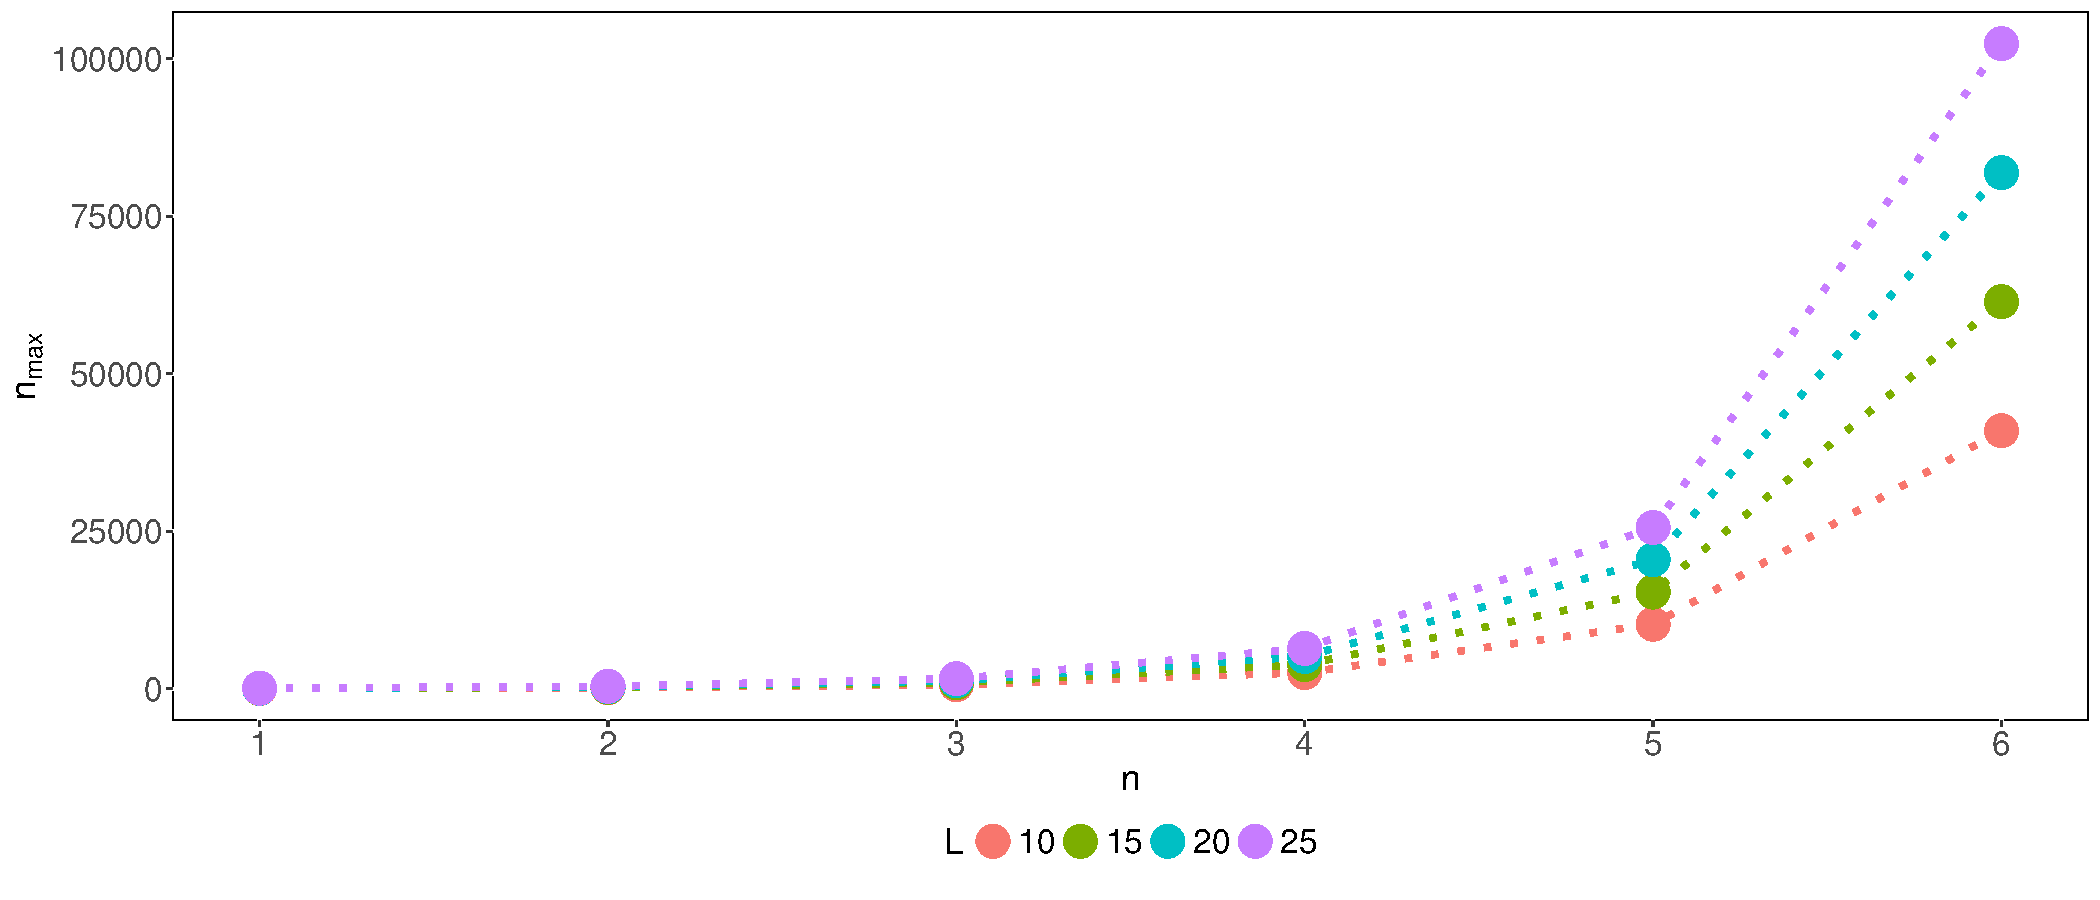
\includegraphics[width=\maxwidth]{figure/unnamed-chunk-4-1} 

}



\end{knitrout}

\end{center}
    \end{block}
    \vfill
    
    \begin{block}{Reducing number of n-grams}
    \begin{figure}
    \centering
    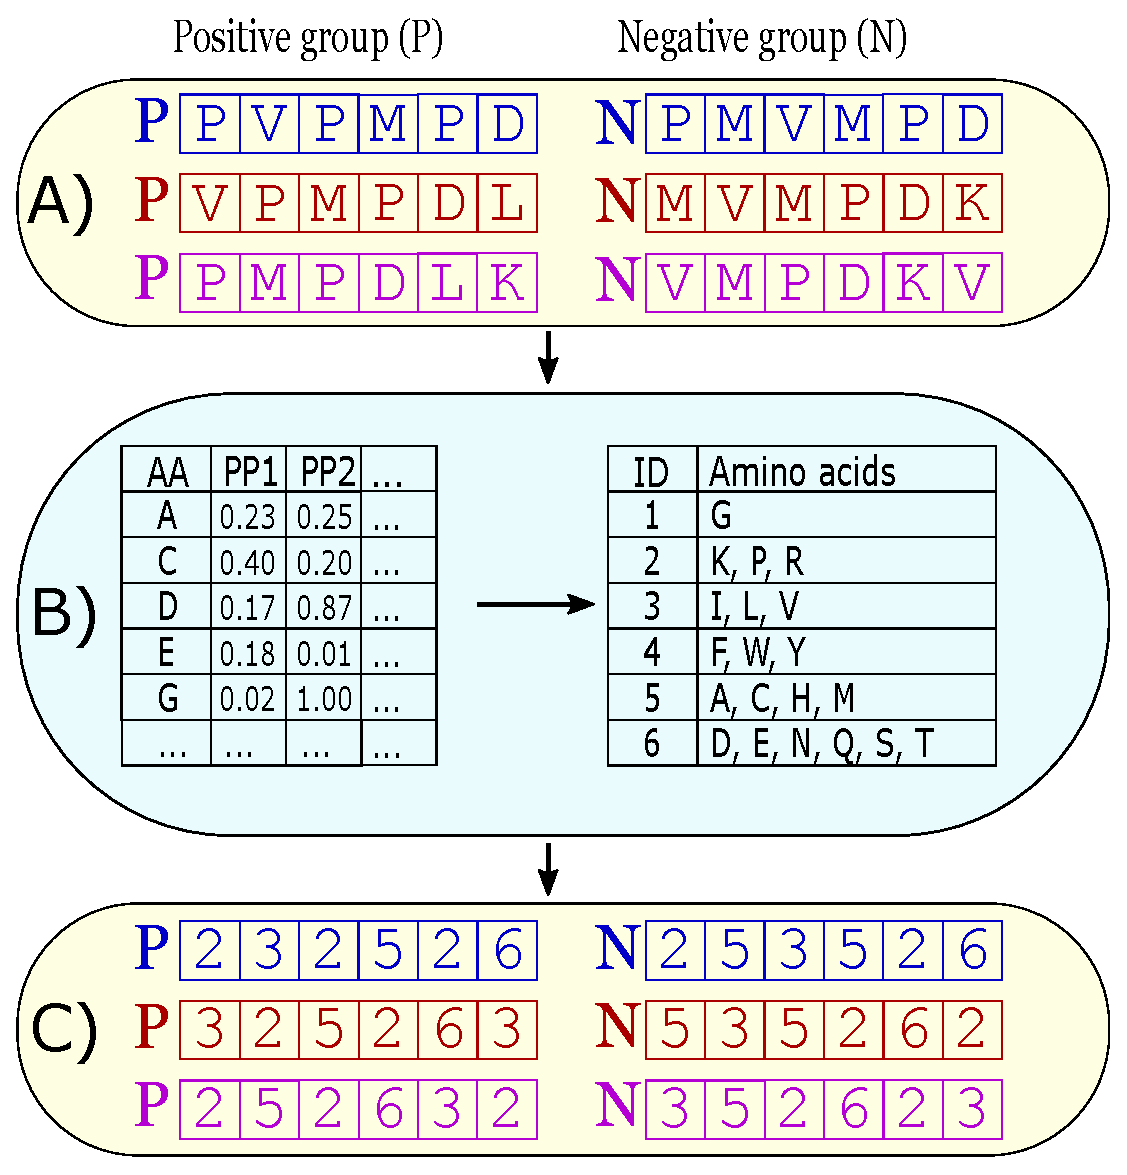
\includegraphics[width=0.5\columnwidth]{biogram_figures/biogram_scheme.eps} 
    \end{figure}

A) Input data: peptides with a known status (e.g. amyloid/nonamyloid). 

B) Creation of an encoding using a combination of physicochemical properties (PP). 

C) Reduction of the amino acid alphabet according to an encoding. The number of possible n-grams is reduced, because $m$ is smaller (e.g. in this case $m$ is reduced from 20 to 6).
      
    \end{block}
    \vfill
 
 \begin{block}{Bibliography}
  \tiny{
  \bibliographystyle{apalike}
  \bibliography{amyloids}
  }
  \end{block}
  \vfill   

}
\end{minipage}
\end{beamercolorbox}
\end{column}


%new column ------------------------------------------------------    

\begin{column}{.51\textwidth}
\begin{beamercolorbox}[center,wd=\textwidth]{postercolumn}
\begin{minipage}[T]{.95\textwidth}  
\parbox[t][\columnheight]{\textwidth}
{






%' \begin{block}{2-gram frequencies in sequences}
%' 
%' <<specSensPlot2, echo = FALSE, message=FALSE, fig.height=8, fig.width=14>>=
%' #ggplot(seq_inter_ct, aes(x = len, y = prop, fill = tar, label = paste0(round(prop, 4) * 100, "%"))) +
%' load("specsens.RData")
%' ggplot(filter(amylo_freq, n == 2), aes(x = variable, y = freq, fill = tar, colour = tar)) +
%'   geom_bar(stat = "identity", position = "dodge") + 
%'   scale_y_continuous("Frequency") +
%'   scale_x_discrete("Group ID\n") + 
%'   scale_fill_manual("Amyloid", values = c("no" = "skyblue", "yes" = "tan2")) +
%'   scale_colour_manual("Amyloid", values = c("no" = "skyblue", "yes" = "tan2")) +
%'   facet_wrap(~ enc, scales = "free_x", ncol = 1) +
%'   guides(colour = FALSE) +
%'   cool_theme
%' @
%' 
%' \end{block}
%' \vfill


    \begin{block}{Selection of important n-grams}
    Model and statistic independent permutation tests can be used to filter features obtained through counting n-grams.
    
    During a permutation test class labels are randomly exchanged during computation of a significance statistic. p-values are defined as:
    
\begin{center}
\scalebox{0.85}{
$      
\textnormal{p-value} = \frac{N_{T_P > T_R}}{N}
$
}
\end{center}

where $N_{T_P > T_R}$ is number of times when $T_P$ (permuted test statistic) was more extreme than $T_R$ (test statistic for non-permuted data).

Permutation tests are computationally expensive (especially considering precise estimation of small p-values, because the number of permutations is inversely proportional to the interval between p-values).

\medskip

\textbf{Qui}ck \textbf{P}ermutation \textbf{T}est (QuiPT) thanks to the unique parameterization replaces a permutation test with the exact two-sided Fisher's test~\citep{lehmann1986testing} reducing the computation cost. 
      
    \end{block}
    \vfill



 
\begin{block}{signalHsmm -  prediction of signal peptides}
Signal peptides are n-terminal guiding sequences with three distinguishable regions: n-, h- and c-region. Using the n-gram approach we created \textit{signalHsmm}, a software for prediction of signal peptides.

\medskip

    \textit{signalHsmm} has two models representing respectively proteins with and without signal peptides. The probabilities of both fits and predicted cleavage site constitute the software output.    
    \begin{figure}
    \centering
    \resizebox{32.5cm}{!}{%
    \begin{tikzpicture}[->,>=stealth',shorten >=2pt,auto,node distance=9.5cm, thick]
      \tikzstyle{line} = [draw=black, color=blue!30!black!50, line width=4.5mm, -latex']
      \tikzstyle{main node} = [circle,fill=blue!20,draw, minimum size = 2.2cm, font=\itshape,
         align=center,  top color=white, bottom color=blue!50!black!70 ] %font=\sffamily\small\bfseries,
      %nodes
      \node[main node]          	(start') 	[]						{Start};	     
      \node[main node, bottom color=purple!70!black!70] 	(nregion') 	[right of=start',xshift=-5mm, yshift=15mm] 	{n-region};
      \node[main node, bottom color=pink!70!black!70] 	(hregion') 	[right of=nregion',xshift=-5mm,yshift=15mm] 	{h-region};
      \node[main node, bottom color=gray!70!black!70] 	(cregion') 	[right of=hregion',xshift=-5mm,yshift=-15mm] 	{c-region};
      \node[main node, bottom color=green!70!black!70] 	(mature') 	[right of=cregion',xshift=-5mm, yshift=-15mm] 	{Mature protein};
      
      %lines
      \path [line] (start')   edge node [left, color=black] {} (nregion');
      \path [line] (nregion') edge node [below, color=black] { } (hregion');
      \path [line] (hregion') edge node [below, color=black] { } (cregion');
      \path [line] (cregion') edge node [left, color=black] { } (mature');
      \draw [line] (start') to[out=340,in=200] (mature');
    \end{tikzpicture} }
    \end{figure}


    \end{block}
    \vfill   

\begin{block}{signalHsmm benchmark}
\begin{table}[ht]
\centering

\begin{tabular}{rllll}
  \toprule
 & Sensitivity & Specificity & MCC & AUC \\ 
  \midrule
signalP 4.1 (no tm) \citep{2011petersensignalp} & 0.8235 & \textbf{0.9100} & 0.6872 & 0.8667 \\ 
   \rowcolor{white}signalP 4.1 (tm) \citep{2011petersensignalp} & 0.6471 & 0.9431 & 0.6196 & 0.7951 \\
   signalHsmm & \textbf{0.9804} & 0.8720 & \textbf{0.7409} & \textbf{0.9262} \\ 
   \rowcolor{white}signalHsmm (raw aa) & 0.8431 & 0.9005 & 0.6853 & 0.8718 \\ 
   \bottomrule
\end{tabular}
\end{table}

Comparison of performance measures for different classifiers according to singal peptide-containing proteins from members of \textit{Plasmodiidae}. 

\medskip

Thanks to the usage of reduced amino acid alphabet, \textit{signalHsmm} better recognizes signal peptides belonging to \textit{Plasmodiidae} which are characterized by an atypical amino acid composition.


\end{block}
\vfill

\begin{block}{AmyloGram}
Amyloids are proteins associated with the number of clinical disorders (e.g., Alzheimer's, Creutzfeldt-Jakob�s and Huntington�s diseases). We created \textit{AmyloGram}, n-based predictor of amyloidogenicity using decision rules extracted by random forests.

\medskip

\begin{table}[ht]
\centering

\begin{tabular}{ccccc}
  \toprule
Classifier & AUC & MCC & Sensitivity & Specificity \\ 
  \midrule
AmyloGram & \textbf{0.8972} & \textbf{0.6307} & 0.8658 & 0.7889 \\ 
  \rowcolor{white}PASTA \citep{walsh_pasta_2014} & 0.8550 & 0.4291 & 0.3826 & 0.9519 \\ 
   FoldAmyloid \citep{garbuzynskiy_foldamyloid:_2010} & 0.7351 & 0.4526 & 0.7517 & 0.7185 \\ 
  \rowcolor{white}APPNN \citep{familia_prediction_2015} & 0.8343 & 0.5823 & \textbf{0.8859} & 0.7222 \\ 
   \bottomrule
\end{tabular}
\end{table}

\end{block}
\vfill



\begin{block}{Summary and funding}
The n-gram analysis creates versatile classifiers able to extract more universal decision rules (e.g. \textit{signalHsmm}, which is able to also predict signal peptides in atypical organisms) or better detect specific proteins. Nonetheless, despite computational quickness provided by the QuiPT method, curse of dimensionality limits n-gram methods to the analysis of shorter sequences.

\bigskip

Our software is avaible as web-servers:

\begin{enumerate}

\item \textit{signalHsmm} web-server: \url{smorfland.uni.wroc.pl/signalHsmm}.

\item \textit{AmyloGram} web-server: \url{smorfland.uni.wroc.pl/amylogram}.

\end{enumerate}

\bigskip

This research was partially funded by the KNOW Consortium and National Science Center (2015/17/N/NZ2/01845).

\end{block}
\vfill




}
\end{minipage}
\end{beamercolorbox}
\end{column}
\end{columns}  
\end{frame}
\end{document}
